% Supplementary Information: Design of PoolParty and StateCounter
% 
% COMPILATION NOTE:
% This document uses the minted package for Python syntax highlighting.
% Compile with: pdflatex -shell-escape si.tex
% Requires Python and Pygments to be installed: pip install Pygments

\documentclass[11pt]{article}

%% ============================================================================
%% PACKAGES
%% ============================================================================

% Page geometry
\usepackage[margin=1in]{geometry}

% Typography
\usepackage[T1]{fontenc}
\usepackage{lmodern}

% Code highlighting with minted
\usepackage{minted}

% Tables
\usepackage{booktabs}
\usepackage{longtable}
\usepackage{array}

% Links and references
\usepackage{hyperref}
\hypersetup{
    colorlinks=true,
    linkcolor=blue,
    urlcolor=blue,
    citecolor=blue
}

% Inline Python code macro using minted
\newcommand{\inpy}[1]{\mintinline{python}{#1}}


% Graphics (if needed for figures)
\usepackage{graphicx}

% Math support
\usepackage{amsmath}
\usepackage{amssymb}

%% ============================================================================
%% MINTED CONFIGURATION
%% ============================================================================

% Set default options for minted code blocks
\setminted{
    fontsize=\small,
    linenos=false,
    frame=single,
    framesep=2mm,
    bgcolor=gray!5,
    breaklines=true
}

% Define a custom style for Python code blocks
\newminted{python}{
    fontsize=\small,
    linenos=true,
    frame=single,
    framesep=2mm,
    bgcolor=gray!5,
    breaklines=true
}

%% ============================================================================
%% DOCUMENT METADATA
%% ============================================================================

\title{Supplemental Information for ``PoolParty:\\Declartive design of commplex oligonucleotide libraries''}
\author{[Author Names]}
\date{\today}

%% ============================================================================
%% DOCUMENT
%% ============================================================================

\begin{document}

\maketitle

\tableofcontents
\newpage

%% ============================================================================
%% SECTION: INTRODUCTION
%% ============================================================================

\section{Introduction}
\label{sec:introduction}

PoolParty makes it easy to design complex libraries involving barcodes, mutagenesis, insertion and deletion scanning, and other common operations. 

The core idea behind PoolPart is that library construction should be \emph{declarative} rather than \emph{imperative}. Rather than explicitly constructing each sequence in the library, users specify high-level operations that, when carried out in series, generated the desired library. After laying out these rules, users simiply specify how many sequence to generate and poolparty takes care of the rest. This approach separates the \emph{what} (library specification) from the \emph{how} (enumeration or sampling), 

Poolparty has two core types of objects: Pools and Operations. A Pool object represents a yet-to-be-realized set of sequences. An Operation object represents a computation that yields a Pool object, and can take zero, one, or multiple Pool objects as input.  To create a sequence library, users first specify the rules for making the library by chaining together a series of Operations, the result of which is a Pool boject. Users then call on that pool to generate the number of desired sequences. 

The following two examples illustrate PoolParty's core capabilities.

\subsection{Example 1: Fixed and Random Mode Operations}
\label{subsec:example-random}

Each component Operation of the computation graph can be in one of four modes: \inpy{'fixed'}, \inpy{'random'}, \inpy{'sequential'}, or \inpy{'hybrid'}.  Fixed mode operations are deterministic: for a given input they always produce the same output. Random mode operation, on the other hand, will generally produce a different output each time they are called due to them having an internal state that changes unpredictably. 

Here is an example of PoolParty code that uses \inpy{'random'} and \inpy{'fixed'} operations to generate the type of construct commonly used in massively parallel reporter assays (MPRAs). First the core sequence elemenets are defined as simple python strings: \inpy{wt_seq} is a regulatory sequence of iterest, \inpy{adapter_5_seq} is a constant-sequence adapter, and \inpy{adapter_3_iupac} is an adapter containing degerate nucleotides that will be used as a barcode. Next, the \inpy{pp.mutagenize()} operation is called on \inpy{wt_seq}, generating a pool \inpy{mut_pool} comprising randomly mutated versions of \inpy{wt_seq}. Next, the \inpy{pp.from_iupac_motif()} operation is called on \inpy{adapter_3_iupac}, generating a pool \inpy{adapter_3_pool} in which the \inpy{N} characters have been replaced by randomly selected DNA nucleotides. Next, the \inpy{pp.join} operation deterministically joins the 3\' adaptor sequence, mutagenized pool, and barcode-containing 5\' adaptor sequence into a final \inpy{oligo_pool_1}. Finally, the \inpy{pp.generate_seqs()} method is called with the desired number of sequence. This produces a pandas dataframe \inpy{df} that lists each sequence along with a ``design card'', i.e.\ a series of fields that describes the decisions each operation made in order to arrive at each resulting sequence. 

\begin{minted}{python}
import poolparty as pp

# Mark changes by changing case of affected bases
pp.set_default('mark_changes',True)

# Define component sequences 
wt_seq  = 'ATCGATCGATATCGATCGAT'        # 10 nt wild-type
ad5_seq = 'GAAC'                        # 3 nt 5' adapter
ad3_seq = 'TGGANNNNNCCAG'               # 3 + 5N barcode + 3

# Create pool of randomly mutagenized wt_seq sequences
mut_pool = pp.mutagenize(wt_seq, num_mutations=3)

# Create pool of 3' adaptors with random barcodes
ad3_pool = pp.from_iupac_motif(ad3_seq, mode='random')

# Join into final oligo pool
oligo_pool = pp.join([ad5_seq, mut_pool, ad3_pool], spacer_str=' ')

# Sample 5 sequences
df = oligo_pool.generate_seqs(num_seqs=5, seed=42)
print(df['seq'])
\end{minted}

Key points:
\begin{itemize}
    \item \inpy{pp.set_default('mark_changes',True)} sets the default option to mark all changes (mutations) in the generated sequences, typically displaying them in a different case for easy identification.
    \item \inpy{pp.mutagenize()} generates a pool of sequences containing different combinations of mutations at within a specified wild-type sequence. Here we instruct poolparty to introduce 3 mutations into each sequence. This operation runs in random mode by default, which means that the specific mutations that each sequence recieves is random. 
    \item \inpy{pp.from_iupac_motif()} generates a pool of sequences derived from an IUPAC sequence, i.e., a DNA sequence in which special characters (such as \'N\') signify degenerate bases. This too runs in random mode by default. 
    \item \inpy{pp.join()} joins together multiple sequences/Pools. It has no variable internal state so always runs in fixed mode. It also takes an argment, \inpy{spacer_str}, which we use here to add a space between the mutagenized region and adaptor sequences. 
    \item \inpy{generate_seqs(num_seqs=N, seed)} instructs \inpy{oligo_pool} to construct $N$ sequences using the specified random seed. It retuns a Pandas dataframe, here called \inpy{df}. The first column is named \inpy{'seq'} and contains the resulting sequences:
    \begin{center}
        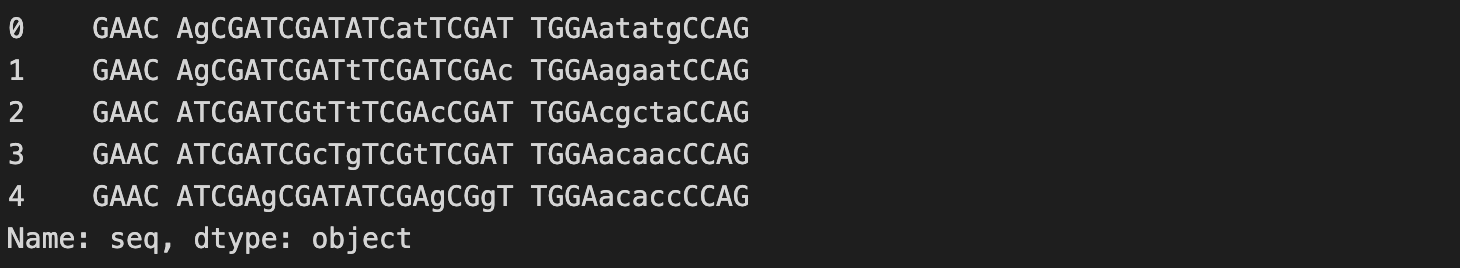
\includegraphics[width=\textwidth]{example1_seqs.png}
    \end{center}
    \item The other columns of the dataframe contain design card information, i.e., the  information that was used to create each sequence variant (Note: columns have been pruned and renamed for simplicity).
    \begin{center}
        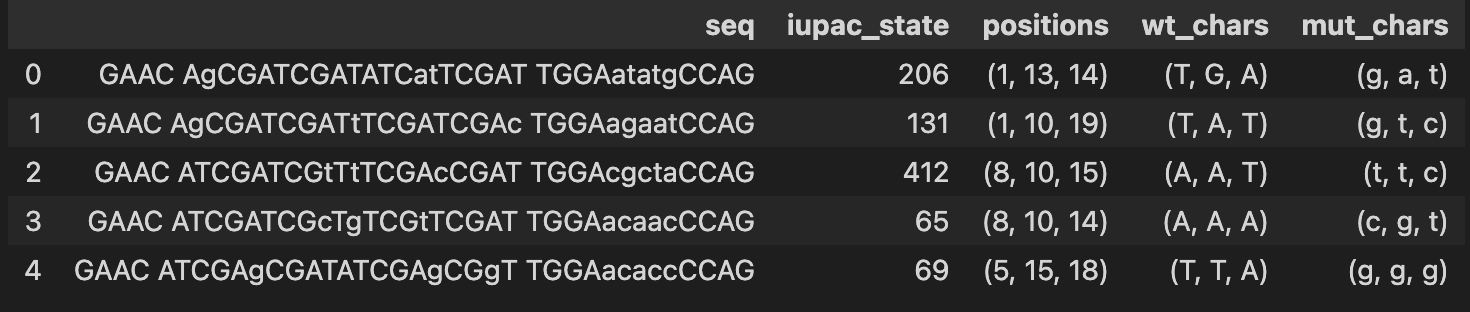
\includegraphics[width=\textwidth]{example1_df.png}
    \end{center}
    \item During the execution of \inpy{oligo_pool.generate_seqs()}, each sequence is computed one-at-a-time using a computation tree that can be visualized by running \inpy{oligo_pool.print_tree()}:
    \begin{center}
        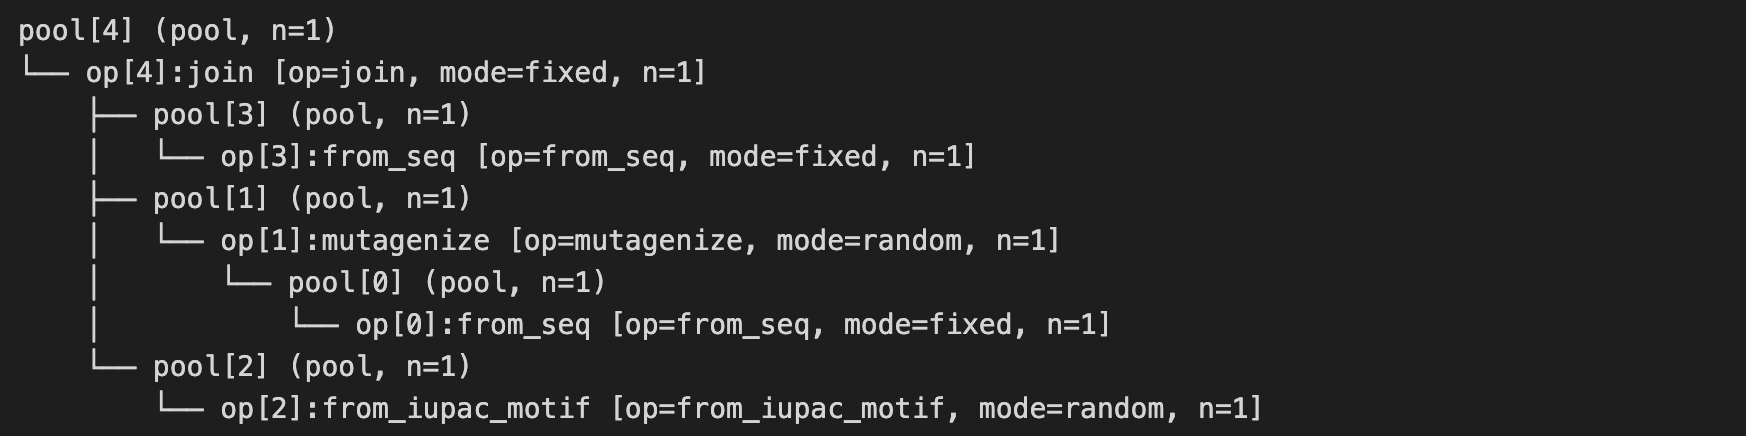
\includegraphics[width=\textwidth]{example1_tree.png}
    \end{center}
\end{itemize}

\subsection{Example 2: Sequential Mode (Cartesian Product + Stack Enumeration)}
\label{subsec:example-sequential}

This example demonstrates sequential enumeration of a combinatorial library. We create 
a replacement scan (with two insert variants at four positions) and a deletion scan, 
then stack them to enumerate all 12 combinations.

\begin{minted}{python}
# Create insert pool with two variants
ins_pool = pp.from_seqs(['AAAAA', 'TTTTT'], mode='sequential')

# Replacement scan at step=5 intervals
rep_scan_pool = pp.replacement_scan(
    wt_seq, ins_pool, 
    positions=range(0, 20, 5),  # [0, 5, 10, 15]
    mode='sequential',
    mark_inserts=True
)

# Deletion scan at same positions
del_scan_pool = pp.deletion_scan(
    wt_seq, 
    deletion_length=5,
    positions=range(0, 20, 5),
    mode='sequential',
    mark_deletions=True
)

# Stack replacement scan and deletion scan (union of states)
combo_scan_pool = pp.stack([rep_scan_pool, del_scan_pool])

# Join into final oligo (reusing adapter_3_pool from above)
oligo_pool_2 = pp.join([adapter_5_seq, combo_scan_pool, adapter_3_pool], spacer_str='.')

# Enumerate all 12 combinations: (2 inserts x 4 positions) + (4 deletions)
df = oligo_pool_2.generate_seqs(num_complete_iterations=1, seed=42)
print(df['seq'].tolist())
\end{minted}

\noindent\textbf{Example output} (12 sequences, all same length, inserts in UPPERCASE):

\begin{minted}[fontsize=\footnotesize]{text}
GAATTC.AAAAAcgatcgatcgatcg.GGATCC.agtcgtatca.CTGCAG  # AAAAA at pos 0
GAATTC.atcgAAAAAcgatcgatcg.GGATCC.tcagctgatc.CTGCAG  # AAAAA at pos 5
GAATTC.atcgatcgAAAAAatcgatcg.GGATCC.gcatgctagc.CTGCAG  # AAAAA at pos 10
GAATTC.atcgatcgatcgAAAAAcg.GGATCC.atcgatcgat.CTGCAG  # AAAAA at pos 15
GAATTC.TTTTTcgatcgatcgatcg.GGATCC.tgcatgcatg.CTGCAG  # TTTTT at pos 0
GAATTC.atcgTTTTTcgatcgatcg.GGATCC.cgatcgatcg.CTGCAG  # TTTTT at pos 5
GAATTC.atcgatcgTTTTTatcgatcg.GGATCC.atgcatgcat.CTGCAG  # TTTTT at pos 10
GAATTC.atcgatcgatcgTTTTTcg.GGATCC.gctagctagc.CTGCAG  # TTTTT at pos 15
GAATTC.-----cgatcgatcgatcg.GGATCC.agtcgtatca.CTGCAG  # del at pos 0
GAATTC.atcg-----cgatcgatcg.GGATCC.tcagctgatc.CTGCAG  # del at pos 5
GAATTC.atcgatcg-----atcgatcg.GGATCC.gcatgctagc.CTGCAG  # del at pos 10
GAATTC.atcgatcgatcg-----cg.GGATCC.atcgatcgat.CTGCAG  # del at pos 15
\end{minted}

Key points:
\begin{itemize}
    \item \mintinline{python}{mode='sequential'} enables deterministic enumeration of all states
    \item Cartesian product: insert variants $\times$ scan positions gives $2 \times 4 = 8$ replacement states
    \item \mintinline{python}{pp.stack()} creates a union of states ($8 + 4 = 12$ total)
    \item \mintinline{python}{mark_inserts=True} highlights inserted sequences in UPPERCASE
    \item \mintinline{python}{generate_seqs(num_complete_iterations=N)} iterates through all states $N$ times
\end{itemize}

\medskip
\noindent The remainder of this document describes the architecture and operations of 
PoolParty and its underlying StateCounter library in detail.


%% ============================================================================
%% SECTION: STATECOUNTER ARCHITECTURE
%% ============================================================================

\section{StateCounter Architecture}
\label{sec:statecounter-architecture}

% TODO: Write this section
%
% This section should describe:
% - The Counter object and its properties (num_states, state, name)
% - The Manager context manager and why it's required
% - Unidirectional state propagation concept
% - How counter algebra enables composable iteration patterns
% - The computation graph / dependency tree structure

[Write description of StateCounter's core architecture, including the Counter class,
Manager context, and unidirectional state propagation mechanism.]

\subsection{Core Concepts}
\label{subsec:statecounter-concepts}

% TODO: Describe key concepts
%
% - Leaf counters: created directly with num_states
% - Derived counters: created through operations on other counters
% - State propagation: setting child state updates all parent states
% - Conflict detection: what happens when incompatible states are assigned

[Describe core concepts: leaf counters, derived counters, state propagation, 
and conflict detection.]

\subsection{The Manager Context}
\label{subsec:manager}

% TODO: Explain the Manager
%
% - Why a context manager is needed
% - What happens when entering/exiting the context
% - How it tracks counter relationships

[Explain the Manager context manager and its role in the StateCounter system.]


%% ============================================================================
%% SECTION: STATECOUNTER OPERATIONS
%% ============================================================================

\section{StateCounter Operations}
\label{sec:statecounter-operations}

% TODO: Write this section
%
% This section should:
% - Provide an overview of available operations
% - Explain the operator overloading (*, +, [], etc.)
% - Reference the table below for quick lookup

[Write overview of StateCounter operations and how they combine counters 
to create complex enumeration patterns.]

% Example table of StateCounter operations
% Modify this table as needed with accurate descriptions

\begin{table}[htbp]
\centering
\caption{StateCounter Operations}
\label{tab:statecounter-ops}
\begin{tabular}{@{}lll@{}}
\toprule
\textbf{Operation} & \textbf{Syntax} & \textbf{Description} \\
\midrule
Product & \mintinline{python}{A * B} & Cartesian product of two counters \\
Stack & \mintinline{python}{stack([A, B])} & Union/sum of counters (one active at a time) \\
Slice & \mintinline{python}{A[start:stop:step]} & Subset of counter states \\
Repeat & \mintinline{python}{A * n} & Repeat counter $n$ times \\
Shuffle & \mintinline{python}{shuffle_counter(A)} & Randomly permute state order \\
Sample & \mintinline{python}{sample_counter(A, k)} & Random sample of $k$ states \\
Synchronize & \mintinline{python}{synchronize_counters(A, B)} & Lock counters to same state \\
Split & \mintinline{python}{split_counter(A, sizes)} & Split counter into parts \\
Interleave & \mintinline{python}{interleave_counters([A, B])} & Interleave states from counters \\
Passthrough & \mintinline{python}{passthrough(A)} & Identity operation (for debugging) \\
\bottomrule
\end{tabular}
\end{table}


%% ============================================================================
%% SECTION: POOLPARTY ARCHITECTURE  
%% ============================================================================

\section{PoolParty Architecture}
\label{sec:poolparty-architecture}

% TODO: Write this section
%
% This section should describe:
% - The Pool object as a sequence generator
% - Lazy evaluation and why it matters for large combinatorial spaces
% - How Pools compose through operations (similar to string operations)
% - The relationship between Pools and their underlying StateCounters
% - Sequential vs random generation modes

[Write description of PoolParty's core architecture, including the Pool class,
lazy evaluation, and how Pools compose to define oligonucleotide libraries.]

\subsection{Pool Composition}
\label{subsec:pool-composition}

% TODO: Describe how pools combine
%
% - Concatenation with +
% - Repetition with *
% - Slicing with []
% - Other composition patterns

[Describe how Pool objects can be composed using string-like operations.]

\subsection{Generation Modes}
\label{subsec:generation-modes}

% TODO: Explain sequential vs random modes
%
% - Sequential mode: enumerate all states in order
% - Random mode: sample states randomly with replacement
% - Hybrid mode: some pools sequential, others random

[Explain the different sequence generation modes available in PoolParty.]


%% ============================================================================
%% SECTION: POOLPARTY OPERATIONS
%% ============================================================================

\section{PoolParty Operations}
\label{sec:poolparty-operations}

% TODO: Write this section
%
% This section should:
% - Categorize operations by type (sequence creation, scanning, modification, etc.)
% - Explain when to use each operation
% - Reference the table below

[Write overview of PoolParty operations and how they enable different 
library design patterns.]

% Example table of PoolParty operations
% This is a representative subset - modify as needed

\begin{longtable}{@{}llp{7cm}@{}}
\caption{PoolParty Operations} \label{tab:poolparty-ops} \\
\toprule
\textbf{Operation} & \textbf{Category} & \textbf{Description} \\
\midrule
\endfirsthead
\multicolumn{3}{c}{\textit{(continued from previous page)}} \\
\toprule
\textbf{Operation} & \textbf{Category} & \textbf{Description} \\
\midrule
\endhead
\midrule
\multicolumn{3}{r}{\textit{(continued on next page)}} \\
\endfoot
\bottomrule
\endlastfoot

% Sequence Creation Operations
\mintinline{python}{from_seq} & Creation & Create pool from a single sequence \\
\mintinline{python}{from_seqs} & Creation & Create pool from multiple sequences \\
\mintinline{python}{from_iupac_motif} & Creation & Create pool from IUPAC ambiguity codes \\
\mintinline{python}{from_prob_motif} & Creation & Create pool from position weight matrix \\
\mintinline{python}{get_kmers} & Creation & Generate all k-mers from alphabet \\
\addlinespace

% Scanning Operations
\mintinline{python}{deletion_scan} & Scanning & Systematic single-position deletions \\
\mintinline{python}{insertion_scan} & Scanning & Systematic single-position insertions \\
\mintinline{python}{replacement_scan} & Scanning & Systematic single-position replacements \\
\mintinline{python}{breakpoint_scan} & Scanning & Scan for breakpoint positions \\
\addlinespace

% Marker Operations
\mintinline{python}{marker_scan} & Marker & Scan for marker positions \\
\mintinline{python}{marker_multiscan} & Marker & Scan multiple markers \\
\mintinline{python}{replace_marker} & Marker & Replace marker with sequence \\
\addlinespace

% Mutagenesis Operations
\mintinline{python}{mutagenize} & Mutagenesis & Apply mutations to sequence \\
\mintinline{python}{mutagenize_orf} & Mutagenesis & Apply codon-aware mutations to ORF \\
\addlinespace

% Sequence Manipulation
\mintinline{python}{join} & Manipulation & Join multiple pools \\
\mintinline{python}{stack} & Manipulation & Stack pools (one active at a time) \\
\mintinline{python}{repeat} & Manipulation & Repeat pool sequence \\
\mintinline{python}{seq_slice} & Manipulation & Slice sequence positions \\
\mintinline{python}{seq_shuffle} & Manipulation & Shuffle sequence order \\
\mintinline{python}{reverse_complement} & Manipulation & Reverse complement sequence \\
\addlinespace

% State Operations
\mintinline{python}{state_slice} & State & Slice pool states \\
\mintinline{python}{state_shuffle} & State & Shuffle pool states \\
\mintinline{python}{state_sample} & State & Sample pool states \\
\mintinline{python}{sync} & State & Synchronize pool states \\

\end{longtable}


%% ============================================================================
%% SECTION: INTEGRATION
%% ============================================================================

\section{Integration Between PoolParty and StateCounter}
\label{sec:integration}

% TODO: Write this section
%
% This section should explain:
% - How each Pool has an underlying Counter
% - How Pool operations map to Counter operations
% - How state propagation enables sequence generation
% - The flow from Pool.generate_library() through counter iteration

[Write description of how PoolParty uses StateCounter internally,
including how Pool operations wrap Counter operations and how 
state propagation enables lazy sequence generation.]


%% ============================================================================
%% SECTION: CODE EXAMPLES
%% ============================================================================

\section{Code Examples}
\label{sec:code-examples}

% This section demonstrates the minted package syntax for including Python code.
% Replace these examples with real examples from PoolParty/StateCounter.

\subsection{StateCounter Example}
\label{subsec:statecounter-example}

The following example demonstrates basic StateCounter usage with the product operation:

\begin{minted}{python}
from statecounter import Counter, Manager

with Manager():
    # Create leaf counters
    A = Counter(num_states=2, name='A')
    B = Counter(num_states=3, name='B')
    
    # Combine with product (Cartesian product)
    C = A * B  # 6 states total
    
    # Iterate and see parent states update
    for state in C:
        print(f"C={state}, A={A.state}, B={B.state}")
\end{minted}

% You can also use inline code like this:
To create a counter, use \mintinline{python}{Counter(num_states=n, name='X')}.


\subsection{PoolParty Example}
\label{subsec:poolparty-example}

The following example demonstrates creating a mutagenesis library with barcodes:

\begin{minted}{python}
from poolparty import Pool

# Define the DNA sequence
seq = "ATCGATCGATCGATCGATCG"

# Create a pool with all single deletions
pool = Pool.from_seq(seq).deletion_scan()

# Add a barcode region
barcode = Pool.get_kmers(length=10, alphabet='ACGT')

# Concatenate to create final library
library = pool + barcode

# Generate sequences
seqs_df = library.generate_library(
    combinatorially_complete_pools=[pool],
    num_complete_iterations=5
)
\end{minted}


\subsection{Advanced Example: Combining Operations}
\label{subsec:advanced-example}

% TODO: Add a more complex example showing multiple operations

\begin{minted}{python}
# Example: Create a library with multiple scanning operations
# [Add your advanced example here]
pass
\end{minted}


%% ============================================================================
%% SECTION: APPENDIX (OPTIONAL)
%% ============================================================================

% Uncomment if you want an appendix
% \appendix
% \section{Additional Details}
% \label{sec:appendix}

% [Optional appendix content]


\end{document}
